\subsection{从 TOP-D 的证明到可验证的泛化}

TOP-D 的三个理论对象是即时奖励乘 score 的二阶矩、算术分布算子的收缩，以及固定奖励 MDP 的性能下界。前两者不能单独保证神经网络的有限 inner 优化或整条 response 的 KL 下降。本节保留有限词表、完整支持和单个固定 teacher，进一步连接精确 target、内层拟合、共同评价散度与轨迹访问测度。所有新增结论在实验前先用解析证明和数值恒等式核验；真实模型的矩测量用于检验实际常数，不替代证明。

\subsection{精确幂均值步降低所有凸生成散度}

令 $s_a=q_a/t_a$。幂均值 target 可写为 $m_a=t_aG(s_a)/Z$，其中
\begin{equation}
 G(s)=[(1-\lambda)s^\kappa+\lambda]^{1/\kappa},\quad
 G_0(s)=s^{1-\lambda},\quad Z=\E_tG(s).
\end{equation}
$G$ 严格递增，$G(s)/s$ 严格递减。对 $\kappa>0$，第二条由
\begin{equation}
 \frac{d}{d\log s}\log\frac{G(s)}s
 =-\frac{\lambda s^{-\kappa}}{1-\lambda+\lambda s^{-\kappa}}<0
\end{equation}
得到；几何端点导数为 $-\lambda$。又有 $Z=\sum_aq_a[G(s_a)/s_a]$，故存在 $s_\star\in[\min s,\max s]$ 使 $G(s_\star)/s_\star=Z$。若 $s_a<s_\star$，则 $s_a\le G(s_a)/Z\le s_\star$；若 $s_a>s_\star$，则 $s_\star\le G(s_a)/Z\le s_a$。

\begin{theorem}[单教师的凸生成散度单调性]
\label{thm:proximal-all-f-divergences}
对任意凸函数 $\varphi:(0,\infty)\to\R$、$\varphi(1)=0$，定义 $D_\varphi(q\Vert t)=\sum_at_a\varphi(q_a/t_a)$。精确 target 满足 $D_\varphi(m\Vert t)\le D_\varphi(q\Vert t)$。因此 $\KL(m\Vert t)$、$\KL(t\Vert m)$、Hellinger 散度、TV 和 $\chi^2(m\Vert t)$ 同时不增加。
\end{theorem}

\begin{proof}
取 $c\in\partial\varphi(s_\star)$。凸函数 $\varphi(s)-cs$ 在 $s_\star$ 取得最小值，且在其两侧分别单调不增、单调不减。每个 $s_a'=m_a/t_a=G(s_a)/Z$ 都位于 $s_a$ 与 $s_\star$ 之间，因此 $\varphi(s_a')-cs_a'\le\varphi(s_a)-cs_a$。乘以 $t_a$ 并求和，由 $\sum_at_as_a'=\sum_at_as_a=1$，线性项抵消，得结论。\hfill$\square$
\end{proof}

这个结论比各自 $D_\kappa$ 的单调性更强，但只直接覆盖精确 target。它并不声称有限 inner 只要降低任何一个拟合损失，就自动同时改善所有散度。

\subsection{保持 teacher 的可逆 Markov 核}

还可构造一个依赖 $q,t$ 的转移核 $K$，满足 $tK=t$、$qK=m$。令 $\delta_a=m_a-q_a$，$L=\{a:\delta_a>0\}$、$H=\{b:\delta_b<0\}$，以及 $D=\sum_{a\in L}\delta_a=\sum_{b\in H}(-\delta_b)$。$D=0$ 时取 $K=I$。否则，对 $a\in L,b\in H$ 定义
\begin{equation}
 w_{ab}=w_{ba}=\frac{\delta_a(-\delta_b)}{D(s_b-s_a)},\qquad
 K_{ab}=w_{ab}/t_a,\quad K_{ba}=w_{ab}/t_b,
\end{equation}
其余非对角项为零，$K_{aa}=1-\sum_{b\ne a}K_{ab}$。由共同交点性质，$a\in L$ 时 $\delta_a/t_a\le s_\star-s_a$，$b\in H$ 时 $(-\delta_b)/t_b\le s_b-s_\star$。所以
\begin{equation}
 \sum_{b\in H}w_{ab}\le\frac{\delta_a}{s_\star-s_a}\le t_a,\qquad
 \sum_{a\in L}w_{ab}\le\frac{-\delta_b}{s_b-s_\star}\le t_b.
\end{equation}
对角项非负，行和为一；$t_aK_{ab}=t_bK_{ba}$ 保证详细平衡与 $tK=t$。对 $a\in L$，$(qK)_a-q_a=\sum_b w_{ab}(s_b-s_a)=\delta_a$；对 $b\in H$ 同样得到其损失质量，故 $qK=m$。

由 $m_j/t_j=\sum_i(t_iK_{ij}/t_j)s_i$ 与 Jensen 不等式，也能重新证明上一条定理。这个核是精确更新的数学表示，不要求实际构造一个词表大小平方的矩阵。它给出共同 teacher 下的保序质量转移解释，避免仅凭某个特定 KL 方向描述更新。

\subsection{目标半径随插值强度单调}

固定 $q,t,\kappa$，记 $m_\lambda$ 为 target。对 $0<\lambda_1<\lambda_2<1$，$m_{\lambda_1}/q$ 随 $\rho=t/q$ 严格递增，且
\begin{equation}
 \frac{m_{\lambda_2,a}}{m_{\lambda_1,a}}
 =\frac{Z_{\lambda_1}}{Z_{\lambda_2}}
 \left(\frac{1-\lambda_2+\lambda_2\rho_a^\kappa}
 {1-\lambda_1+\lambda_1\rho_a^\kappa}\right)^{1/\kappa}
\end{equation}
也随 $\rho_a$ 严格递增。几何端点对应 $Z_{\lambda_1}\rho_a^{\lambda_2-\lambda_1}/Z_{\lambda_2}$。取两条比率相等的共同交点，$m_{\lambda_2}/q$ 相对 $m_{\lambda_1}/q$ 在低端进一步减小、高端进一步增大。用上一条定理的支撑直线证明反向不等式，得到
\begin{equation}
 D_\varphi(m_{\lambda_2}\Vert q)\ge D_\varphi(m_{\lambda_1}\Vert q).
\end{equation}
$\lambda_1=0$ 时由散度非负性成立。取 $\varphi(s)=(\sqrt s-1)^2$，得 Hellinger 距离与 Fisher--Rao 距离随 $\lambda$ 单调。对不同 prefix 的固定加权平均也成立。因此可以在指定前缀面板上唯一校准共同的目标半径，而不是假设相同 $\lambda$ 自动等于相同步幅。校准面板与实际比较面板不同时，半径还须在比较面板上独立读出。

\subsection{有限 inner 的 reverse KL 与 Rényi 证书}

令 $\epsilon=\KL(p\Vert m)$、$A(a)=\log(m_a/t_a)$，$H=\max A-\min A$。恒等式为
\begin{equation}
 \KL(p\Vert t)=\epsilon+\KL(m\Vert t)+\sum_a(p_a-m_a)A(a).
\end{equation}
减去 $A$ 的区间中点后使用 Hölder 和 Pinsker 不等式，得到
\begin{equation}
 \KL(p\Vert t)\le\KL(m\Vert t)+\epsilon+H\sqrt{\epsilon/2}.
 \label{eq:proximal-range-certificate}
\end{equation}
若右侧不超过 $\KL(q\Vert t)$，则原始 teacher reverse KL 下降。这里 $H$ 可被极小概率的尾部主导，故还需要一个按概率加权的证书。

对任意 $u>0$，令 $r_u(a)=m_a^{1+u}t_a^{-u}/C_u$，$C_u=\sum_am_a^{1+u}t_a^{-u}$。由
\begin{equation}
 \KL(p\Vert r_u)=\epsilon-u\E_pA+\log C_u\ge0,
\end{equation}
得到
\begin{equation}
 \boxed{\KL(p\Vert t)\le
 \inf_{u>0}\left[(1+1/u)\KL(p\Vert m)+D_{1+u}^{\mathrm R}(m\Vert t)\right]},\quad
 D_{1+u}^{\mathrm R}(m\Vert t)=\frac1u\log C_u.
 \label{eq:proximal-renyi-certificate}
\end{equation}
有限个正 $u$ 上取最小值仍是有效上界。$u\to0$ 时，$D_{1+u}^{\mathrm R}(m\Vert t)=\KL(m\Vert t)+\tfrac u2\Var_mA+O(u^2)$。对固定分布、小拟合误差的局部展开，最优平衡项约为 $\sqrt{2\epsilon\Var_mA}$，解释了概率加权证书为何可能比区间界更紧；有限 $u$ 的精确式才是保证。相同 $u$ 下先逐 prefix 应用再固定测度求平均，也能得到整体条件目标的上界。

\subsection{共同目标下的局部最优形状}

令 $r=\log(t/q)$，$w_\kappa=(\rho^\kappa-\E_q\rho^\kappa)/\kappa$，$w_0=C_qr$，于是 $v_\kappa=qw_\kappa$。对固定 Fisher 速度的单位方向 $u_\kappa=v_\kappa/\|v_\kappa\|_F$，reverse KL 的一阶下降量为
\begin{equation}
 -\nabla\KL(q\Vert t)^\top u_\kappa
 =\frac{\E_q[rw_\kappa]}{\sqrt{\E_qw_\kappa^2}}
 \le\sqrt{\Var_qr}.
\end{equation}
这是 Cauchy--Schwarz 不等式，几何形状 $\kappa=0$ 取得等号。对 forward KL，同样有
\begin{equation}
 -\nabla\KL(t\Vert q)^\top u_\kappa
 =\frac{\E_q[\rho w_\kappa]}{\sqrt{\E_qw_\kappa^2}}
 \le\sqrt{\Var_q\rho},
\end{equation}
算术形状 $\kappa=1$ 取得等号。更一般地，$\kappa$ 自己对应的散度具有自己的自然梯度最陡方向。这个局部确定性最优性与平方根形状的最坏矩性质是不同标准，不能由有界方差推出对任何共同评价目标的最优收敛速度。

\subsection{目标自然速度的锐上界与另一个极小极大形状}

对 $0<\kappa<1/2$，令 $X=\rho^\kappa$、$r=1/\kappa>2$，则 $\E_qX^r=1$。$L^p$ 插值不等式给出
\begin{equation}
 \E_qX^2\le(\E_qX)^{(r-2)/(r-1)}
 =(\E_qX)^{(1-2\kappa)/(1-\kappa)}.
\end{equation}
令 $a=\E_qX\in[0,1]$，$\gamma=(1-2\kappa)/(1-\kappa)$。于是 $\Var_qX\le a^\gamma-a^2$。驻点满足 $a^{2-\gamma}=\gamma/2$，代回并记 $b=(1-2\kappa)/[2(1-\kappa)]$，得到锐上界
\begin{equation}
 \boxed{\sup_{q,t}\|v_\kappa\|_F^2
 =C_{\mathrm{vel}}(\kappa)
 =\frac{b^{1-2\kappa}(1-b)}{\kappa^2}}.
\end{equation}
锐性由 $q=(b,1-b)$、$t\to(1,0)$ 达到：$X$ 仅取 $b^{-\kappa}$ 与零，插值不等式和驻点条件同时成立。完整支持分布以极限逼近这个值。$\kappa=1/2$ 的上确界为 4；$\kappa=0$ 或 $\kappa>1/2$ 无有限上界。

在优化 $b$ 后使用包络导数，$d\log C_{\mathrm{vel}}/d\kappa=-2/\kappa-2\log b$。唯一最小点满足
\begin{equation}
 \log\frac{1-2\kappa_\star}{2(1-\kappa_\star)}=-\frac1{\kappa_\star}.
\end{equation}
左侧加 $1/\kappa$ 的导数为 $-1/[(1-2\kappa)(1-\kappa)]-1/\kappa^2<0$，在零点附近趋于正无穷，在 $1/2$ 附近趋于负无穷，故根唯一。根和常数由第一方参考函数 \texttt{minimax\_velocity\_shape}、\texttt{worst\_fisher\_speed\_squared} 计算并验证。

这个最优形状针对 target 的最坏 Fisher 速度上界，与内层误差相关噪声常数的最优 $\kappa_{\mathrm{fit}}=1/2$ 是不同标准。更小的最大速度不自动代表更快学习；部分 teacher 方向也可能变慢。实验将这个由理论确定的 target 作为独立条件，而不把平方根的简洁闭式性质当作通用最优性。

\begin{figure}[htbp]
 \centering
 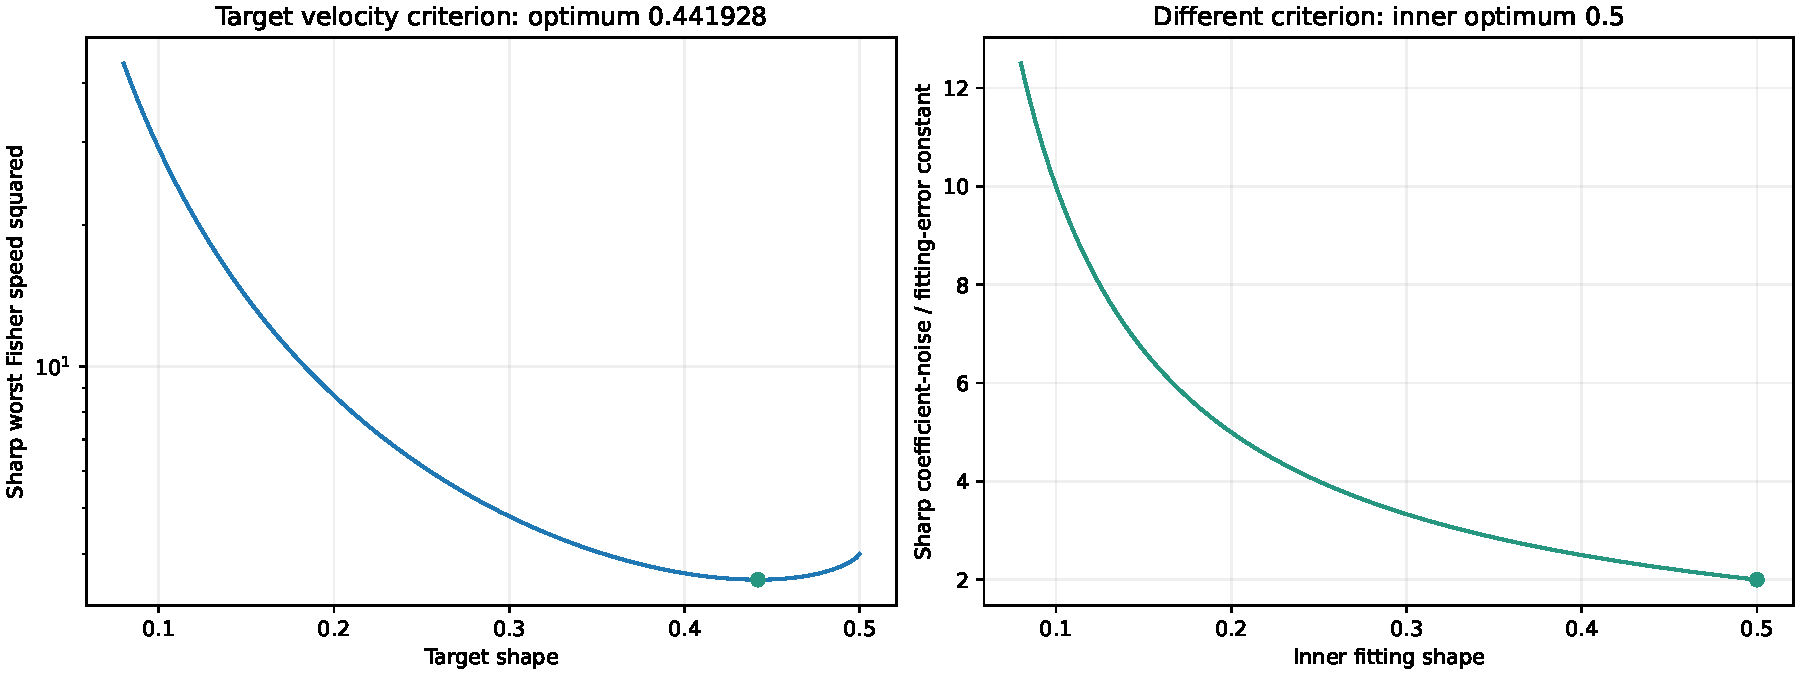
\includegraphics[width=\textwidth]{../../results/power-mean-20261013/two-minimax-criteria.pdf}
 \caption{两个明确而不同的极小极大标准。左图是 target 速度的锐上界，最小点为 $0.441928$；右图是下一小节拟合噪声与损失的锐相对常数 $1/\kappa_{\mathrm{fit}}$，最小点为 $1/2$。二者都不直接等于最高任务准确率。}
\end{figure}

\subsection{方差最优 baseline 与信号归一化}

固定 $p=q$，score 满足 $\E_q\psi=0$。对 $g_b=(f-b)\psi$，均值不依赖 action 无关的 $b$，方差最小化等价于最小化 $\E_q[(f-b)^2\|\psi\|^2]$。微分给出
\begin{equation}
 b_\star=\frac{\E_q[f\|\psi\|^2]}{\E_q\|\psi\|^2},\qquad
 \Var(g_b)-\Var(g_{b_\star})=\E_q\|\psi\|^2(b-b_\star)^2.
\end{equation}
所以 reward 条件均值一般不是方差最优 baseline。categorical logits 的 score 范数平方为 $1-2q_a+\sum_bq_b^2$，完整词表下可精确计算这个最优值。内层 $p\ne q$ 且使用重要性权重 $\omega=p/q$ 时，对 $\omega(f-b)\psi_p$ 的最优 baseline 则用 $\omega^2\|\psi_p\|^2$ 加权。

按相同局部信号斜率比较时，使用 $f/\lambda$。上节的最坏二阶矩阶数于是变成 $\Theta_\kappa(\lambda^{\min\{2,1/\kappa\}-2})$：平方根及更小正形状为 $\Theta(1)$，算术端点为 $\Theta(1/\lambda)$。这说明稳健差异没有被统一尺度归一化完全消除。但实际信号的均值、梯度平方与相对噪声也须同时报告；实际 NN 的 score 范数和内层重要性比率还需额外矩条件。

\begin{figure}[htbp]
 \centering
 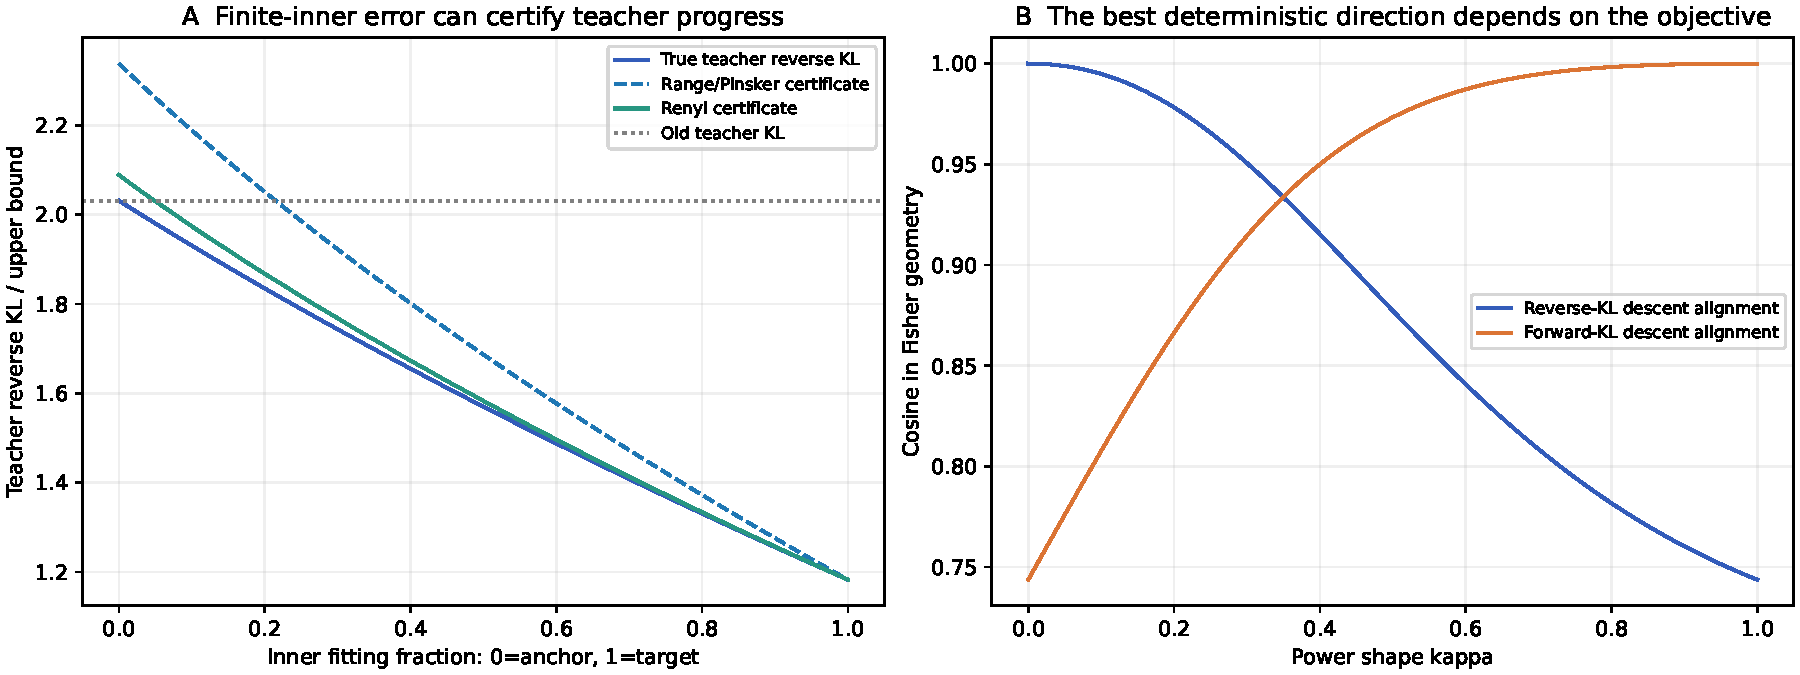
\includegraphics[width=\textwidth]{../../results/power-mean-20261013/inner-certificate-and-direction.pdf}
 \caption{左图将内层拟合误差转为 teacher reverse KL 的区间与 Rényi 上界；右图在相同 Fisher 速度下比较共同评价目标的方向。几何与算术分别对 reverse 与 forward KL 具有局部最陡性质。}
\end{figure}

本节的 Markov 核、半径单调性、有限 inner 证书与方向计算由 \path{experiments/analysis/power_generalization.py} 核验。大模型前缀、四卡训练与预注册判据见实验报告的幂均值部分；数学保证、真实 logit 协方差和实际全参数梯度分别报告。
